\documentclass[12pt,letterpaper]{article}
\usepackage{graphicx,textcomp}
\usepackage{natbib}
\usepackage{setspace}
\usepackage{fullpage}
\usepackage{color}
\usepackage[reqno]{amsmath}
\usepackage{amsthm}
\usepackage{fancyvrb}
\usepackage{amssymb,enumerate}
\usepackage[all]{xy}
\usepackage{endnotes}
\usepackage{lscape}
\newtheorem{com}{Comment}
\usepackage{float}
\usepackage{hyperref}
\newtheorem{lem} {Lemma}
\newtheorem{prop}{Proposition}
\newtheorem{thm}{Theorem}
\newtheorem{defn}{Definition}
\newtheorem{cor}{Corollary}
\newtheorem{obs}{Observation}
\usepackage[compact]{titlesec}
\usepackage{dcolumn}
\usepackage{tikz}
\usetikzlibrary{arrows}
\usepackage{multirow}
\usepackage{xcolor}
\newcolumntype{.}{D{.}{.}{-1}}
\newcolumntype{d}[1]{D{.}{.}{#1}}
\definecolor{light-gray}{gray}{0.65}
\usepackage{url}
\usepackage{listings}
\usepackage{color}

\definecolor{codegreen}{rgb}{0,0.6,0}
\definecolor{codegray}{rgb}{0.5,0.5,0.5}
\definecolor{codepurple}{rgb}{0.58,0,0.82}
\definecolor{backcolour}{rgb}{0.95,0.95,0.92}

\lstdefinestyle{mystyle}{
	backgroundcolor=\color{backcolour},   
	commentstyle=\color{codegreen},
	keywordstyle=\color{magenta},
	numberstyle=\tiny\color{codegray},
	stringstyle=\color{codepurple},
	basicstyle=\footnotesize,
	breakatwhitespace=false,         
	breaklines=true,                 
	captionpos=b,                    
	keepspaces=true,                 
	numbers=left,                    
	numbersep=5pt,                  
	showspaces=false,                
	showstringspaces=false,
	showtabs=false,                  
	tabsize=2
}
\lstset{style=mystyle}
\newcommand{\Sref}[1]{Section~\ref{#1}}
\newtheorem{hyp}{Hypothesis}

\title{Problem Set 2}
\date{Due: February 19, 2023 - Marcus Ó Faoláin, 16327268}
\author{Applied Stats II}


\begin{document}
	\maketitle
	\section*{Instructions}
	\begin{itemize}
		\item Please show your work! You may lose points by simply writing in the answer. If the problem requires you to execute commands in \texttt{R}, please include the code you used to get your answers. Please also include the \texttt{.R} file that contains your code. If you are not sure if work needs to be shown for a particular problem, please ask.
		\item Your homework should be submitted electronically on GitHub in \texttt{.pdf} form.
		\item This problem set is due before 23:59 on Sunday February 19, 2023. No late assignments will be accepted.
	%	\item Total available points for this homework is 80.
	\end{itemize}

	
	%	\vspace{.25cm}
	
%\noindent In this problem set, you will run several regressions and create an add variable plot (see the lecture slides) in \texttt{R} using the \texttt{incumbents\_subset.csv} dataset. Include all of your code.

	\vspace{.25cm}
%\section*{Question 1} %(20 points)}
%\vspace{.25cm}
\noindent We're interested in what types of international environmental agreements or policies people support (\href{https://www.pnas.org/content/110/34/13763}{Bechtel and Scheve 2013)}. So, we asked 8,500 individuals whether they support a given policy, and for each participant, we vary the (1) number of countries that participate in the international agreement and (2) sanctions for not following the agreement. \\

\noindent Load in the data labeled \texttt{climateSupport.csv} on GitHub, which contains an observational study of 8,500 observations.

\begin{itemize}
	\item
	Response variable: 
	\begin{itemize}
		\item \texttt{choice}: 1 if the individual agreed with the policy; 0 if the individual did not support the policy
	\end{itemize}
	\item
	Explanatory variables: 
	\begin{itemize}
		\item
		\texttt{countries}: Number of participating countries [20 of 192; 80 of 192; 160 of 192]
		\item
		\texttt{sanctions}: Sanctions for missing emission reduction targets [None, 5\%, 15\%, and 20\% of the monthly household costs given 2\% GDP growth]
		
	\end{itemize}
	
\end{itemize}

\newpage
\noindent Please answer the following questions:

\begin{enumerate}
	\item
	Remember, we are interested in predicting the likelihood of an individual supporting a policy based on the number of countries participating and the possible sanctions for non-compliance.
	\begin{enumerate}
		\item [] Fit an additive model. Provide the summary output, the global null hypothesis, and $p$-value. Please describe the results and provide a conclusion.
		%\item
		%How many iterations did it take to find the maximum likelihood estimates?
	\end{enumerate}
	
	\item
	If any of the explanatory variables are significant in this model, then:
	\begin{enumerate}
		\item
		For the policy in which nearly all countries participate [160 of 192], how does increasing sanctions from 5\% to 15\% change the odds that an individual will support the policy? (Interpretation of a coefficient)
%		\item
%		For the policy in which very few countries participate [20 of 192], how does increasing sanctions from 5\% to 15\% change the odds that an individual will support the policy? (Interpretation of a coefficient)
		\item
		What is the estimated probability that an individual will support a policy if there are 80 of 192 countries participating with no sanctions? 
		\item
		Would the answers to 2a and 2b potentially change if we included the interaction term in this model? Why? 
		\begin{itemize}
			\item Perform a test to see if including an interaction is appropriate.
		\end{itemize}
	\end{enumerate}
	\end{enumerate}

\newpage
	\section*{Question 1}

\noindent[] Fit an additive model. 
\\\\

\noindent In order to fit an additive model, we use the following code in R studio, with a + instead of a * in order to generate an additive rather than an interactive model. 
\\
\begin{verbatim}
logistic <- glm(choice ~ sanctions + countries, climateSupport, family = "binomial")
\end{verbatim}

\noindent Provide the summary output, the global null hypothesis, and $p$-value. 
\\\\

\noindent Using the summary() function, we can get a summary output as follows:

\begin{verbatim}
summary(logistic)
\end{verbatim}

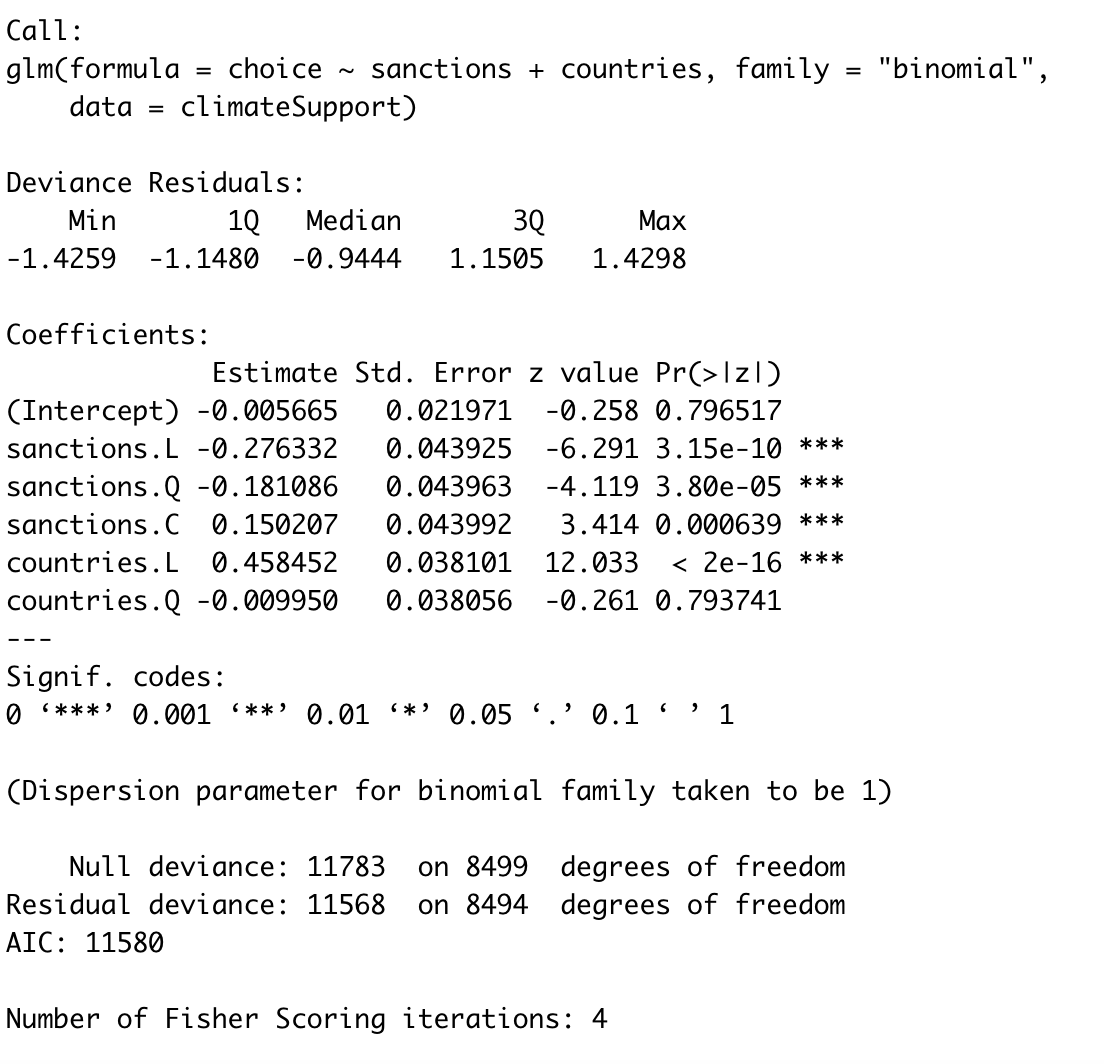
\includegraphics{logreg_output.png}
\newpage

\noindent 
The global null hypothesis ($H_0$) states that none of the coefficients ($\beta$) of the logistic regression model have an influence on the dependent variable "choice". In more literal terms, this means that neither the level of sanctions for non enforcement nor the number of countries that have signed up for the policy has an effect on the binary dependent variable of whether people support the policy or not. 
\\

\noindent In mathematical terms, it looks as follows:
\\\\
$H_0:$ $\beta_1 = \beta_2 = \beta_3 = ... = \beta_n = 0$
\\

\noindent Where each $\beta$ is a coefficient for each of the independent variables in relation to the outcome variable. This means that each $\beta$ would have a slope equal to 0.
\\

\noindent The alternative hypothesis ($H_\alpha$) is that at least one of the $\beta$ coefficients is not equal to and therefore has an influence on the outcome variable.
\\\\
$H_\alpha:$ $\beta_j \neq 0 $
\\

\noindent 
As we can see, four of the $\beta$ coefficients have p-values less than 0.01. This means that we reject the global null hypothesis that all 


\noindent Please describe the results and provide a conclusion.
\\

\noindent 
The coefficient estimate $\beta_1$ in the case of "sanctions.:L" has a value of -0.276332. We can see from the three stars on the table and from the p-value of 3.15e-10 that the result is associated with a p-value of less than 0.05, which suggests that "sanction.L" does in fact have an influence on whether an individual supports an international environmental agreement.
\\\\
\noindent
Going from no sanctions up to 5\% sanctions multiplies the odds of support for an international agreement by $e^-0.276332$, which is equivalent to 0.758561.
\\\\
\noindent 
This means that a change from no sanctions to 5\% sanctions decreases the odds of support for an international agreement by around 24.1\%, when all other factors are controlled for.
\\\\

\noindent We notice from the regression table that the coefficients of sanctions.Q (15\%), sanctions.c (20\%) and countries.L (80/192) are significant. We can interpret these coefficients similarly to the previous one. 
\\\\
\noindent
Going from 5\% sanctions up to 15\% sanctions multiplies the odds of support for an international agreement by $e^-0.181086$, which is equivalent to 0.8343636.
\\\\
\noindent 
This means that a change from 5\% sanctions to 15\% sanctions decreases the odds of support for an international agreement by around 16.6\%, when all other factors are controlled for.

\noindent
\\\\
Going from 15\% sanctions up to 20\% sanctions multiplies the odds of support for an international agreement by $e^0.150207$, which is equivalent to 1.162075.
\\\\
\noindent 
This means that a change from 15\% sanctions to 20\% sanctions increases the odds of support for an international agreement by around 16.2\%, when all other factors are controlled for.
\\\\
\noindent
When the countries supporting it increases from 20/192 to 80/192, the odds in support of the international agreement are multiplied by $e^0.458452$, which is equivalent to 1.581624.
\\\\
\noindent 
This means that when the number of countries supporting an international agreement increases from 20/192 to 80/192, it results, on average, in a 58.2\% increase in the odds of support for the international agreement.
\\\\
\noindent
The p-value of the final coefficient for countries.Q (160/192 countries) is not below 0.05, and therefore we cannot reject the null hypothesis that it has an influence on the dependent variable, choice.
\\\\

\noindent
In conclusion, using the output table, we can create an equation for predicting the odds of support for an international environmental agreement, with the following formula
\\\\
$ ln(\frac{P(Y_i = 1)}{(1 - P(Y_i = 1))}) = \beta_0 + \beta_1X_1 + \beta_2X_2 + \beta_3X_3 + \beta_4X_4$
\\\\

\noindent By subbing in our values, we can get the following equation:
\\\\
$ ln(\frac{P(Y_i = 1)}{(1 - P(Y_i = 1))}) = -0.05 -0.276332X_1 + -0.181086X_2 + 0.150207X_3 + 0.458452X_4$
\\\\

\noindent Which can then be transformed into:
\\\\

$ P(Y_i = 1) = \frac{exp( -0.05 -0.276332X_1 + -0.181086X_2 + 0.150207X_3 + 0.458452X_4)}{1 + exp( -0.05 -0.276332X_1 + -0.181086X_2 + 0.150207X_3 + 0.458452X_4)}$
\\\\
\noindent We can set up a function in R to calculate different odds for us as follows:

\begin{verbatim}
p <- function(x1, x2, x3, x4){
	p <- exp(-0.05 - 0.276332*x1 -0.181086*x2 + 0.150207*x3 + 0.458452*x4)
	q <- 1- exp(-0.05 - 0.276332*x1 -0.181086*x2 + 0.150207*x3 + 0.458452*x4)
	return(p/q)
}
\end{verbatim}

\newpage
\section*{Question 2}

\noindent
If any of the explanatory variables are significant in this model, then:
\\\\

\noindent 
We use the following code to get the predicted probabilities

\begin{verbatim}

predicted_data <- with(climateSupport, expand.grid(countries = unique(countries),
sanctions = unique(sanctions)))

predicted_data <- cbind(predicted_data, predict(logistic4, 
newdata = predicted_data,
type = "response",
se = TRUE))
\end{verbatim}

\noindent Which yields the following output:

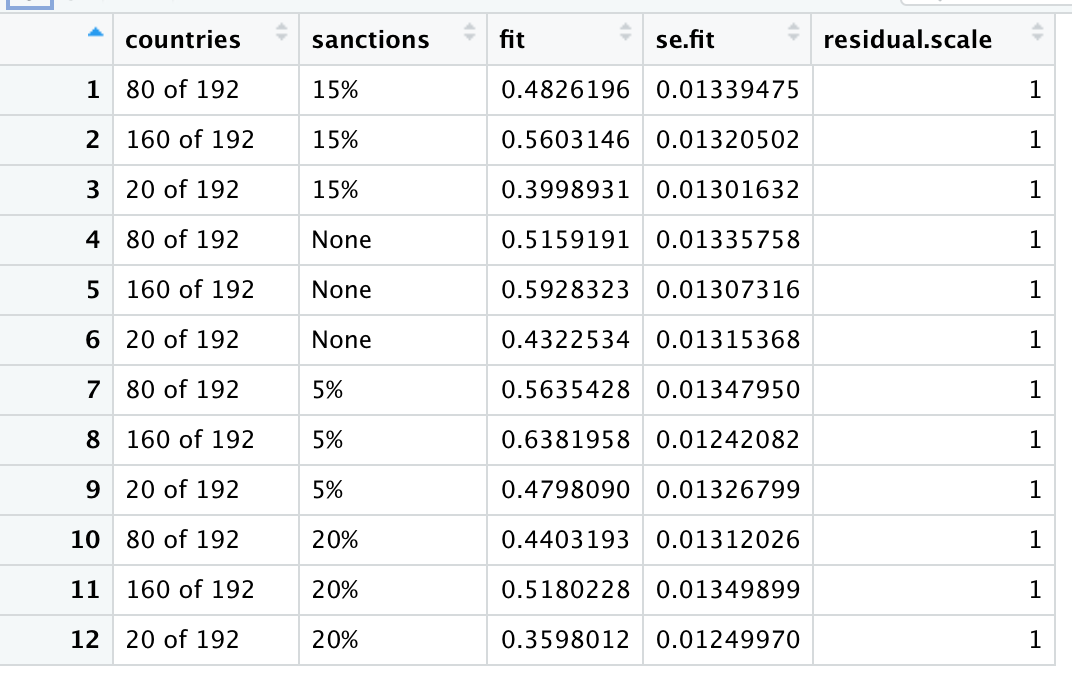
\includegraphics{predicted probabilities.png}


\noindent
	2. (a) For the policy in which nearly all countries participate [160 of 192], how does increasing sanctions from 5\% to 15\% change the odds that an individual will support the policy? (Interpretation of a coefficient)
\\\\
\noindent Increasing sanctions from 5\% to 15\% will multiply the odds of supporting the agreement by $e^181086$, which is equivalent to 0.834636. This means that it will decrease the odds of supporting an international agreement by around 16.5\%.
\\\\

\noindent	
2. (b) For the policy in which very few countries participate [20 of 192], how does increasing sanctions from 5\% to 15\% change the odds that an individual will support the policy? (Interpretation of a coefficient)
\\
\noindent 
Increasing sanctions from 5\% to 15\% changes the odds decreasing it 8\% based on the predicted probabilities table.

\newpage
\noindent
2. (c) What is the estimated probability that an individual will support a policy if there are 80 of 192 countries participating with no sanctions? 
\\\\

\noindent
We can see from the table that the predicted probability support for a policy at 160 countries with no sanctions is 0.5928323, which is around 59.2\%
\\\\
\newpage
\noindent
2. (d) Would the answers to 2a and 2b potentially change if we included the interaction term in this model? Why? 
\\
\noindent The answers would change if we included an interaction term in the model, however, as shown in the following question, it is not appropriate to use an interaction term in the model. The probability would change by the exponent of the relevant interaction terms on page 13.

\newpage
\noindent 2. (e) Perform a test to see if including an interaction is appropriate.
\\
\noindent 
\\
One way we can check to see if an interaction term is by running another logistic regression model with an interaction term instead of an additive term. We can do this and examine the output as follows:

\begin{verbatim}
interaction_log <- glm(choice ~ sanctions*countries,
climateSupport,
family = "binomial")

summary(interaction_log)
\end{verbatim}

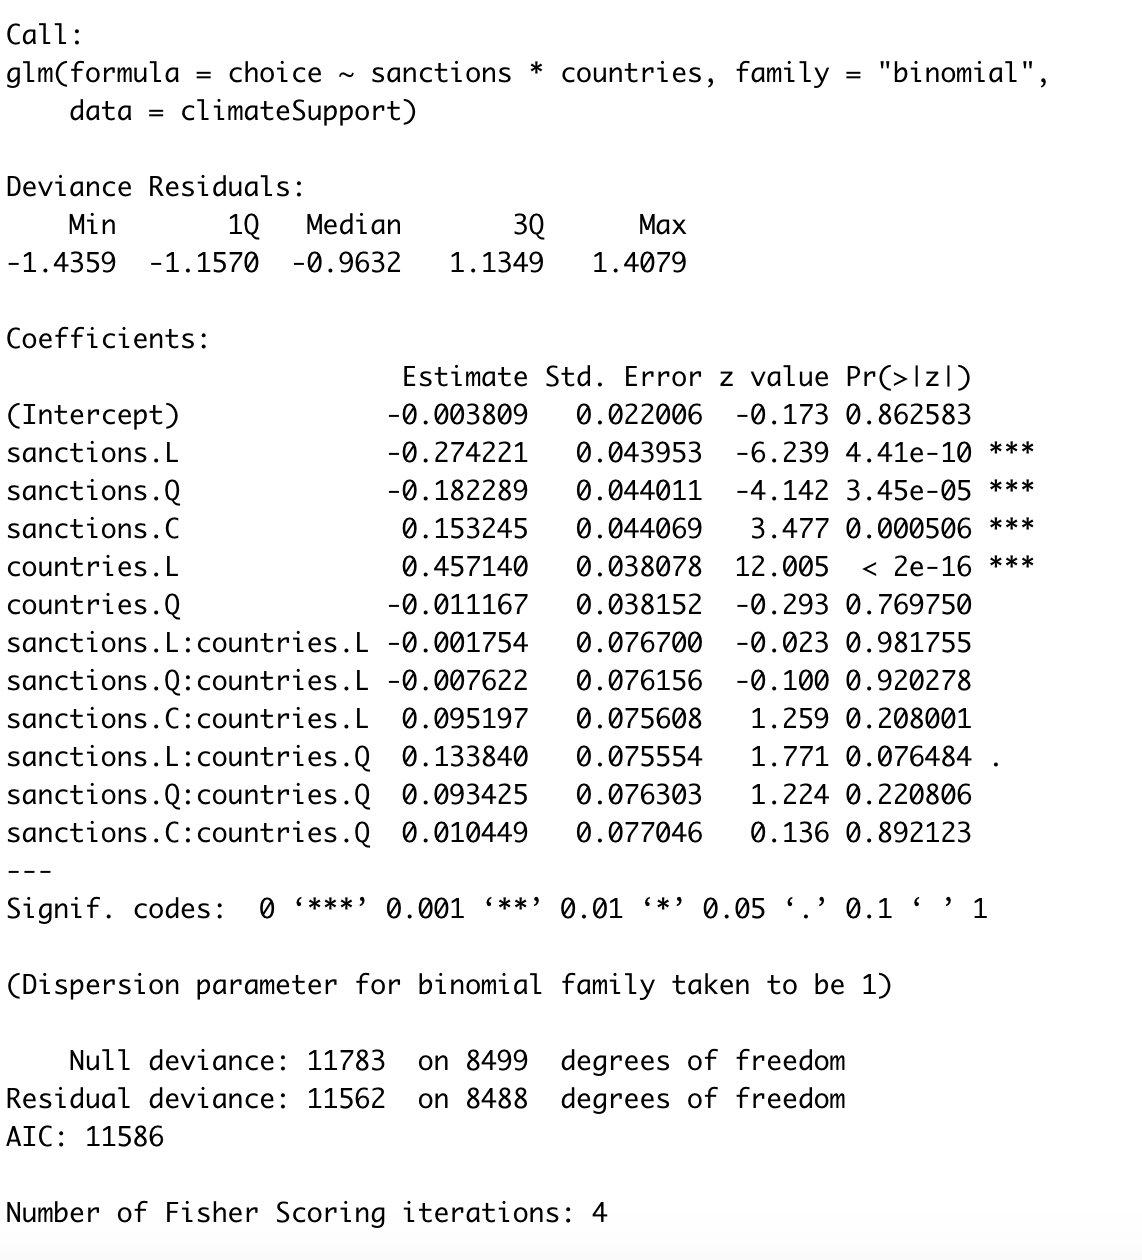
\includegraphics{reg_interactive_output.png}

\noindent
We can see that none of the interative terms have p-values below 0.05. This strongly suggests that the interaction is not a statistically reliable relationship, and we cannot reject the null hypothesis that the interaction between the variables has no effect.
\\\\
\noindent Therefore we can conclude that an interaction is not appropriate in our model. 

\end{document}